\documentclass[a4paper,10pt]{article}
\usepackage[utf8]{inputenc}
\usepackage{graphicx}
\usepackage{fancyvrb}
\usepackage{amsmath}
%\usepackage{mathtools}
\usepackage{color}
\usepackage{float}
\usepackage{hyperref}
\usepackage{tikz}


\title{\textbf{Working notes} \includegraphics[width=1cm]{/export/users/pierre/Images/Rlogo.png}\\ggplot2 implementation of the graphical functions of the ade4 package\\(in working!)}
\author{P.BADY}
\date\today




% paramter for tikz and organization and format of the diagrams
\usetikzlibrary{arrows,shapes,positioning,shadows,trees}
\tikzset{
  basic/.style  = {draw, text width=2cm, drop shadow, font=\sffamily, rectangle},
  root/.style   = {basic, rounded corners=2pt, thin, align=center,
                   fill=green!30},
  level 2/.style = {basic, rounded corners=6pt, thin,align=center, fill=green!60,
                   text width=8em},
  level 3/.style = {basic, thin, align=left, fill=pink!60, text width=6.5em}
}
% end

\usepackage{Sweave}
\begin{document}
\Sconcordance{concordance:ggade4.tex:ggade4.Rnw:%
1 17 1 1 9 13 1 1 0 54 1 1 24 26 0 1 2 2 1 1 2 1 0 1 4 6 0 1 2 5 1 1 2 1 0 %
2 1 3 0 1 2 3 1 1 2 1 0 4 1 4 0 1 2 8 1 1 2 1 0 8 1 1 2 1 0 2 1 4 0 1 2 10 %
1 1 2 1 0 13 1 4 0 1 2 14 1 1 2 1 0 9 1 4 0 1 2 12 1 1 2 1 0 10 1 4 0 1 2 7 %
1 1 2 1 0 10 1 4 0 1 2 11 1 1 2 1 0 11 1 4 0 1 2 6 1 1 2 1 0 11 1 4 0 1 2 7 %
1 1 16 18 0 1 2 3 1 1 2 1 0 13 1 1 4 3 0 2 1 5 0 1 3 10 1 1 8 7 0 1 9 11 0 %
1 2 4 1 1 2 1 0 1 2 1 0 2 1 1 3 2 0 5 1 4 0 1 2 7 1 1 2 1 0 1 2 1 0 2 1 1 3 %
2 0 5 1 4 0 1 2 10 1 1 2 1 0 10 1 4 0 1 2 8 1 1 2 1 0 10 1 4 0 1 2 8 1 1 2 %
1 0 10 1 4 0 1 2 12 1 1 2 1 0 9 1 3 0 1 2 24 1 1 2 54 0 2 1 3 0 1 2 1 1}

\definecolor{Soutput}{rgb}{0,0,0.56}
\definecolor{Sinput}{rgb}{0.56,0,0}
\DefineVerbatimEnvironment{Sinput}{Verbatim}
{formatcom={\color{Sinput}},fontsize=\footnotesize, baselinestretch=0.75}
\DefineVerbatimEnvironment{Soutput}{Verbatim}
{formatcom={\color{Soutput}},fontsize=\footnotesize, baselinestretch=0.75}
% Code de Duncan Murdoch post sur R-help le 07-MARS-2008 :
% This removes the extra spacing after code and output chunks in Sweave,
% but keeps the spacing around the whole block.
\DefineVerbatimEnvironment{GenericCode}{Verbatim}
{fontsize=\footnotesize, baselinestretch=0.75,frame=single}
\fvset{listparameters={\setlength{\topsep}{0pt}}}
\renewenvironment{Schunk}{\vspace{\topsep}}{\vspace{\topsep}}


\maketitle


\newlength\tindent
\setlength{\tindent}{\parindent}
\setlength{\parindent}{0pt}
\renewcommand{\indent}{\hspace*{\tindent}}


\rule{\linewidth}{.5pt}
\begin{center}
\begin{minipage}{0.9\textwidth}
% police par defaut verbatim
\fontfamily{\ttdefault}\selectfont
License: GPL version 2 or newer

Copyright (C) 2000-2021  Pierre Bady

This program/document is free software; you can redistribute it and/or modify it under the terms of the GNU General Public License as published by the Free Software Foundation; either version 2 of the License, or (at your option) any later version.

This program/document is distributed in the hope that it will be useful, but WITHOUT ANY WARRANTY; without even the implied warranty of MERCHANTABILITY or FITNESS FOR A PARTICULAR PURPOSE.  See the GNU General Public License for more details.
\end{minipage}\;
\end{center}
\rule{\linewidth}{.5pt}


\tableofcontents


\section{Motivations}

The objectives of this documment are to propose elements and alternatives for \texttt{ggplot2} implementation (\cite{ggplot2}) of the graphical function from R package ADE-4 (\cite{ade4_2004,ade4_2007a,ade4_2007b}). why ggplot2 ?


\section{Gestion of the limits}

A function \texttt{getLimits} is written to extract the limits of the axes x and y as done in the \texttt{R} package \texttt{ade4}.

\begin{Schunk}
\begin{Sinput}
  getLimits <- function (dfxy, xax=1, yax=2,include.origin=TRUE,origin=c(0,0)){
 	df <- data.frame(dfxy)
 	if (!is.data.frame(df)) 
 		stop("Non convenient selection for df")
 	if ((xax < 1) || (xax > ncol(df))) 
 		stop("Non convenient selection for xax")
 	if ((yax < 1) || (yax > ncol(df))) 
 		stop("Non convenient selection for yax")
 	x <- df[, xax]
 	y <- df[, yax]
 	x1 <- x
 	if (include.origin) 
 		x1 <- c(x1, origin[1])
 	x1 <- c(x1 - diff(range(x1)/10), x1 + diff(range(x1))/10)
 	xlim <- range(x1)
 	
 	y1 <- y
 	if (include.origin) 
 		y1 <- c(y1, origin[2])
 	y1 <- c(y1 - diff(range(y1)/10), y1 + diff(range(y1))/10)
 	ylim <- range(y1)
 	return(list(xlim=xlim, ylim=ylim))
 }
\end{Sinput}
\end{Schunk}

Example for a futur prototype of the function \texttt{ggade} (or \texttt{ggscatter}?)

\begin{Schunk}
\begin{Sinput}
  require(ggplot2)
  ggade <- function(dfxy,xax=1,yax=2,...,include.origin=TRUE,origin=c(0,0)){
   yxlim <- getLimits(dfxy,xax=xax,yax=yax,include.origin=include.origin,origin=origin)
   ggplot(....) + coord_cartesian(xlim=yxlim$xlim,ylim=yxlim$ylim) + coord_fixed(ratio=1)
 }
\end{Sinput}
\end{Schunk}


\section{Representations of the variables}



\begin{Schunk}
\begin{Sinput}
  data(deug)
  deug0 <- dudi.pca(deug$tab, center = deug$cent, scale = FALSE, scan = FALSE)
  deug1 <- dudi.pca(deug$tab, center = TRUE, scale = TRUE, scan = FALSE)
\end{Sinput}
\end{Schunk}


\begin{figure}[H]
\begin{center}
\begin{Schunk}
\begin{Sinput}
  require(ggplot2)
  gg <- ggplot(data=data.frame(eig=deug1$eig,nf=1:length(deug1$eig)), aes(x=nf, y=eig)) 
  gg <- gg + geom_bar(stat="identity") + ggtitle("Eigenvalues from PCA") 
  gg <- gg + ylab("Eigenvalues") + xlab("axis") + theme_light() 
  gg
\end{Sinput}
\end{Schunk}
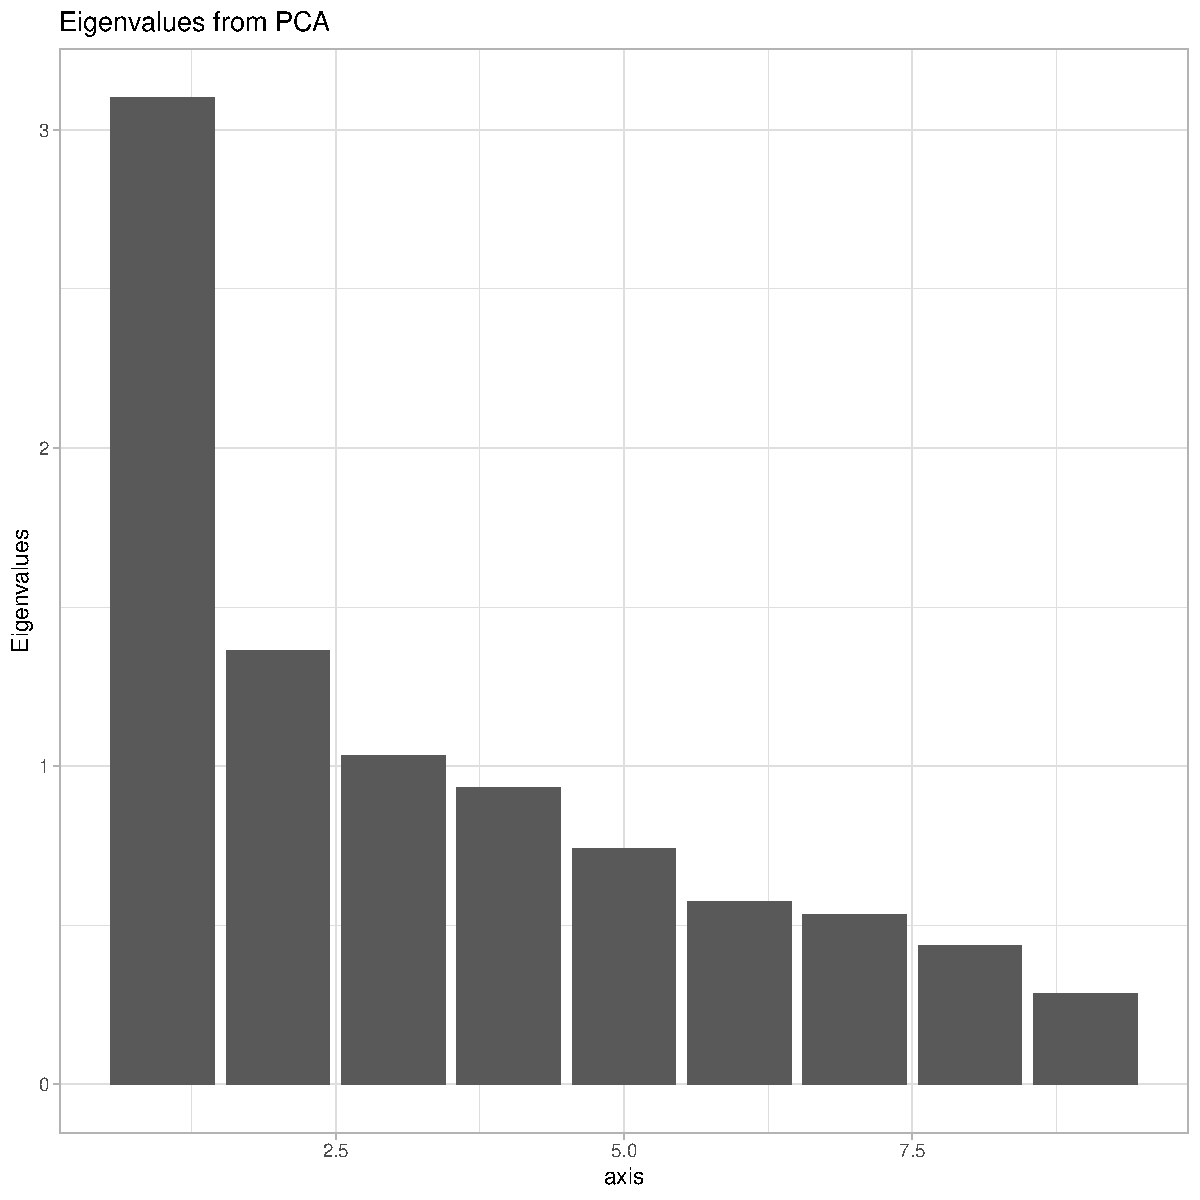
\includegraphics{figs/sweave-eigen1}
\caption{Representation of the Eigenvalues from PCA on correlation matrix}
\label{fig:eigen1}
\end{center}
\end{figure}



\begin{figure}[H]
\begin{center}
\begin{Schunk}
\begin{Sinput}
  require(cowplot)
  require(ggplot2)
  require(ggrepel)
  auxi <- deug0$co
  auxi$label <- rownames(auxi)
  ggx <- ggplot(data=auxi,aes(Comp1,Comp2,label=label) )
  ggx <- ggx + geom_hline(yintercept = 0)+geom_vline(xintercept = 0)
  ggx <- ggx + xlab("axis 1") + ylab("axis 2")
  ggx <- ggx + geom_segment(aes(x=0,xend =Comp1, y=0,yend = Comp2),arrow = arrow(length = unit(0.2,"cm")))
  ggx <- ggx + geom_label_repel(size = 3.5,segment.alpha=0.7,segment.color = "darkgrey",
                               fontface = 'bold',col="black")
  ggx <- ggx + theme_bw() + coord_fixed(ratio=1)
  ggx
\end{Sinput}
\end{Schunk}
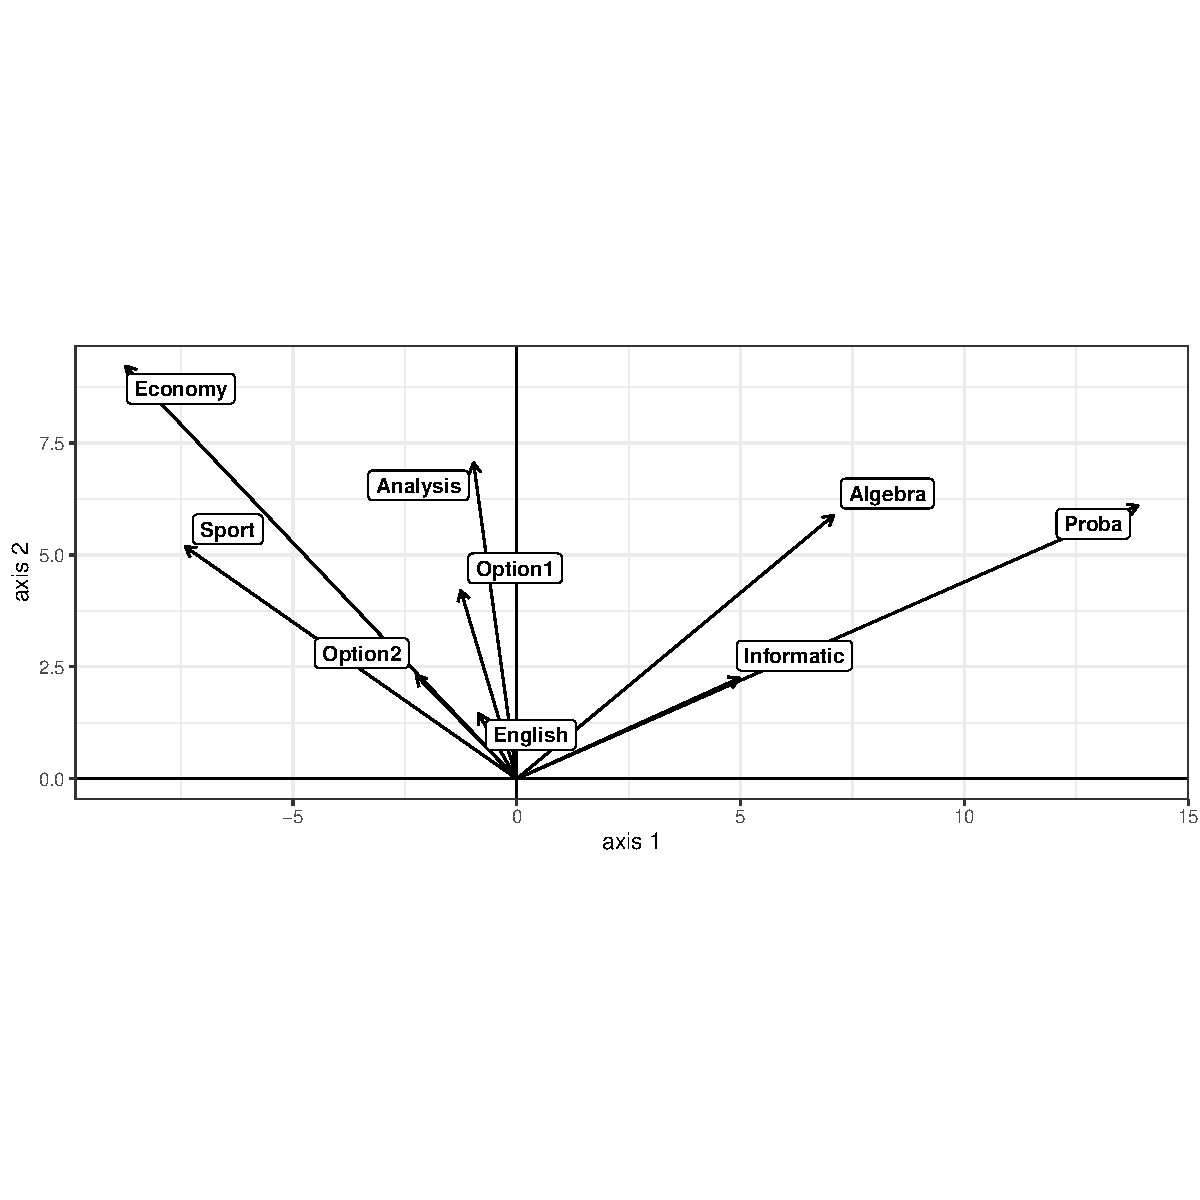
\includegraphics{figs/sweave-coarrow}
\caption{Representation of the variables with correlation circle for PCA on covariance}
\label{fig:coarrow}
\end{center}
\end{figure}





\begin{figure}[H]
\begin{center}
\begin{Schunk}
\begin{Sinput}
  require(cowplot)
  require(ggplot2)
  require(ggrepel)
  require(ggforce)
  auxi <- deug1$co
  auxi$label <- rownames(auxi)
  ggx <- ggplot(data=auxi,aes(Comp1,Comp2,label=label) )
  ggx <- ggx + geom_hline(yintercept = 0)+geom_vline(xintercept = 0)
  ggx <- ggx + xlab("axis 1") + ylab("axis 2")
  ggx <- ggx + geom_circle(data=data.frame(x0=0,y0=0),aes(x0=x0, y0=y0, r=1),inherit.aes = FALSE)
  ggx <- ggx + geom_segment(aes(x=0,xend =Comp1, y=0,yend = Comp2),arrow = arrow(length = unit(0.2,"cm")))
  ggx <- ggx + geom_label_repel(size = 3.5,segment.alpha=0.7,segment.color = "darkgrey",fontface = 'bold',col="black")
  ggx <- ggx + theme_bw() + coord_fixed(ratio=1)
  ggx
\end{Sinput}
\end{Schunk}
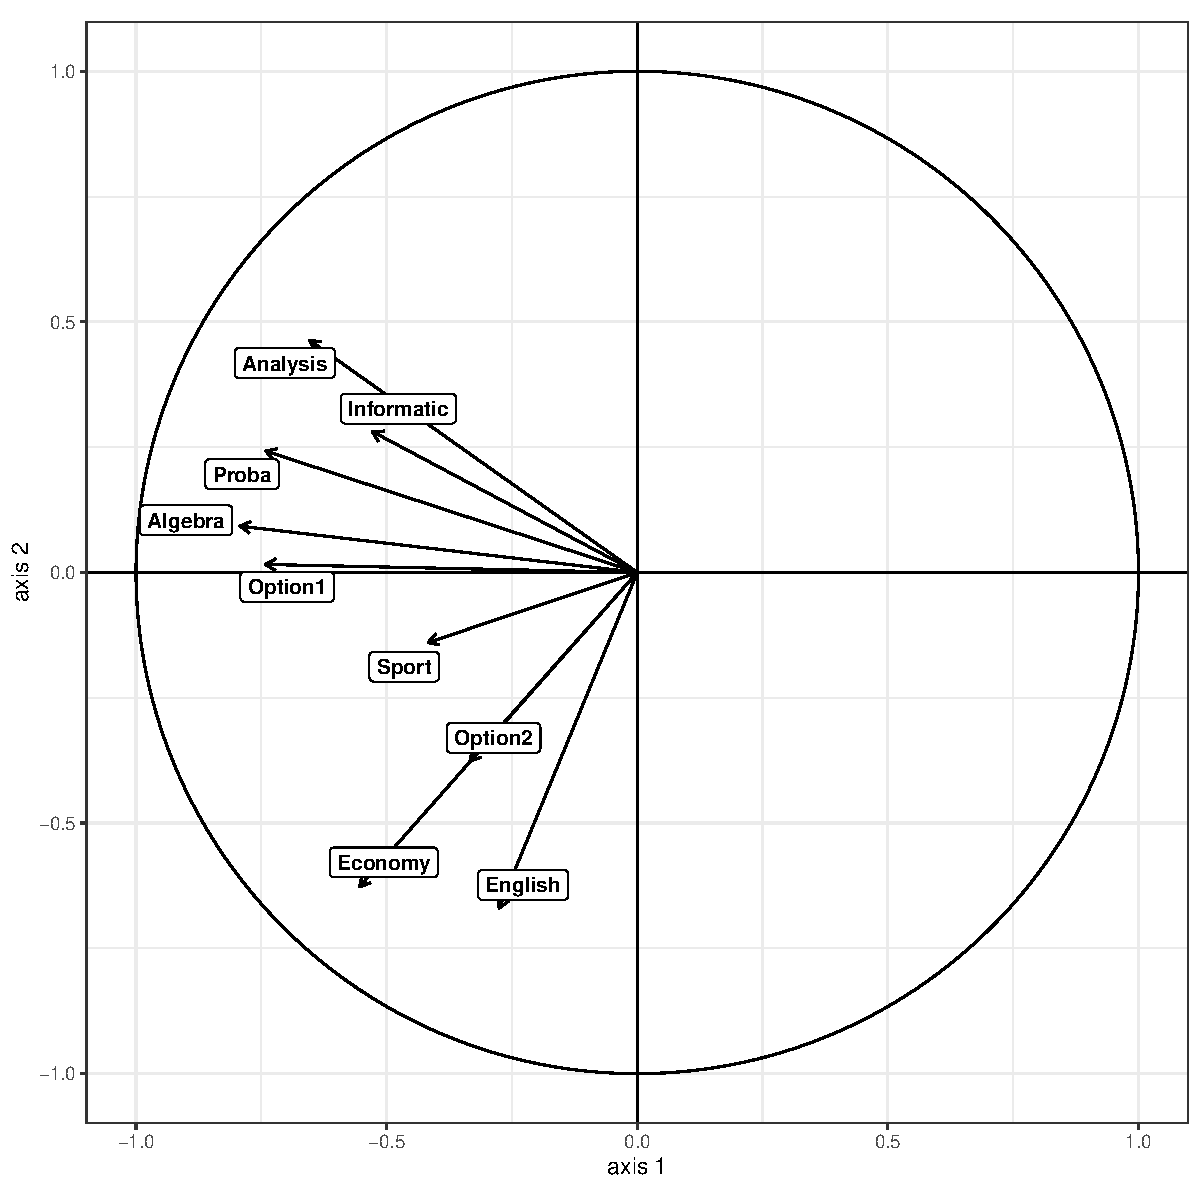
\includegraphics{figs/sweave-cocircle}
\caption{Representation of the variables with correlation circle for PCA on correlation}
\label{fig:cocircle}
\end{center}
\end{figure}





\section{Representations of samples}

representation of the samples on the first factorial plan

\begin{figure}[H]
\begin{center}
\begin{Schunk}
\begin{Sinput}
  require(ggplot2)
  require(ggrepel)
  auxi <- deug1$li
  auxi$label <- rownames(auxi)
  gg <- ggplot(auxi,aes(Axis1,Axis2,label=label))
  gg <- gg + geom_hline(yintercept = 0) + geom_vline(xintercept = 0)
  gg <- gg + geom_point(shape=19,size=3)
  gg <- gg + geom_label_repel(size = 3,segment.alpha=0.7,segment.color = "darkgrey")
  gg <-  gg + theme_bw()+ coord_fixed(ratio=1)
  gg
\end{Sinput}
\end{Schunk}
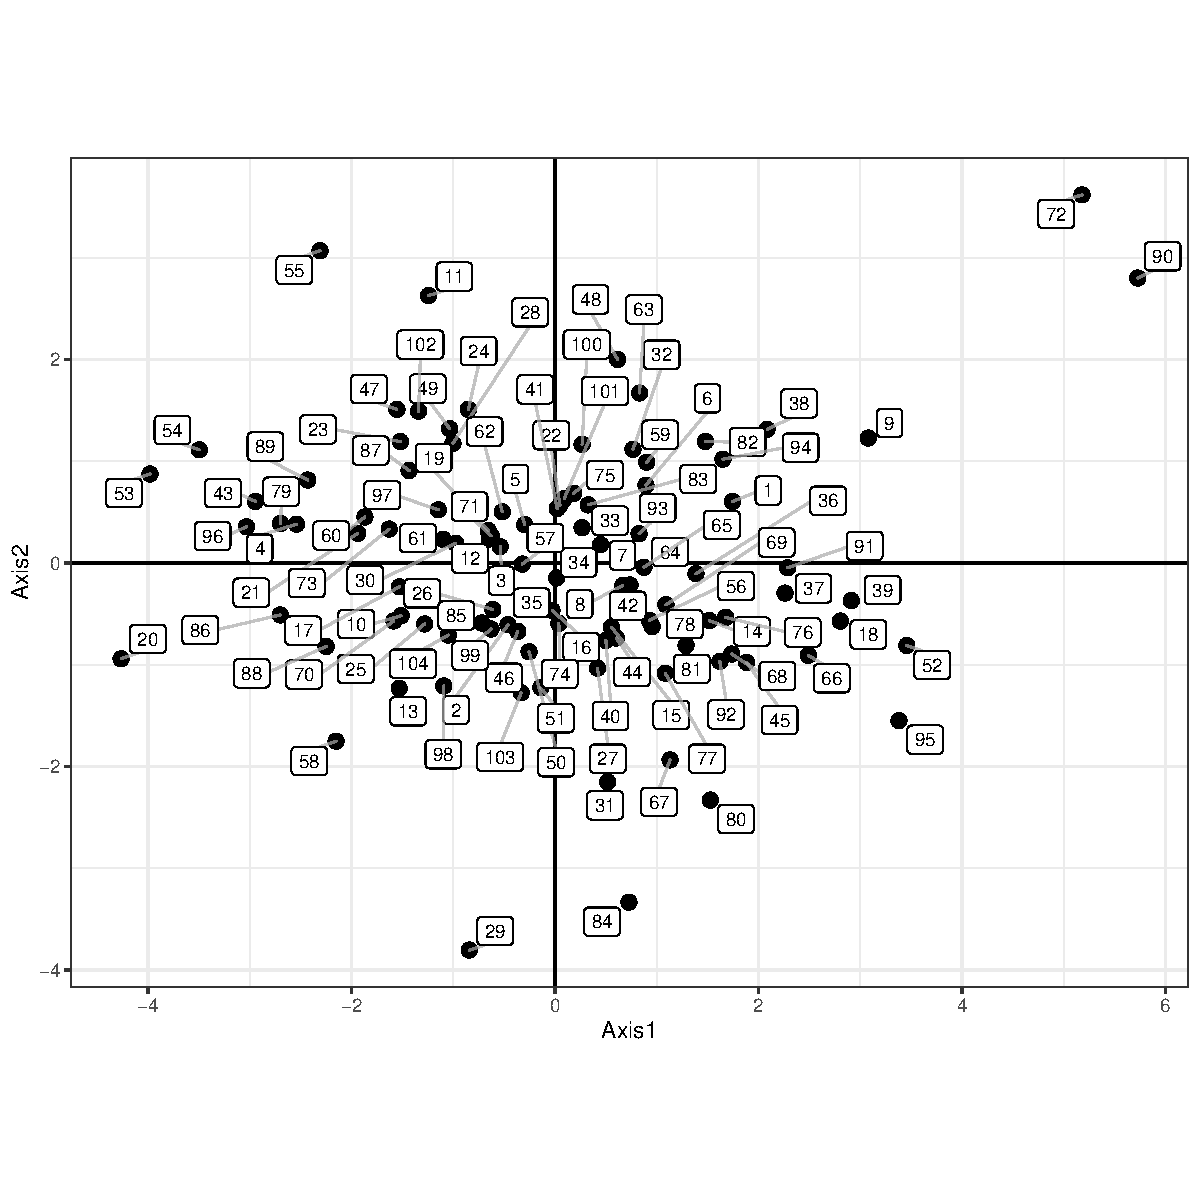
\includegraphics{figs/sweave-lilabel}
\caption{Representation of the observation of the first vectorial plan}
\label{fig:lilabel}
\end{center}
\end{figure}


\section{Representations of samples by group}
\subsection{separated Representations of samples by group}

Representation of the samples on the first factorial plan

\begin{figure}[H]
\begin{center}
\begin{Schunk}
\begin{Sinput}
  require(ggplot2)
  require(ggrepel)
  auxi <- deug1$li
  auxi$label <- rownames(auxi)
  auxi$group <- substring(as.character(deug$result),1,1)
  gg <- ggplot(auxi,aes(Axis1,Axis2,label=label))
  gg <- gg + geom_hline(yintercept = 0) + geom_vline(xintercept = 0)
  gg <- gg + geom_point(shape=19,size=3)
  gg <- gg + geom_label_repel(size = 3,segment.alpha=0.7,segment.color = "darkgrey")
  gg <-  gg + theme_bw() + coord_fixed(ratio=1) + facet_wrap(~ group) 
  gg
\end{Sinput}
\end{Schunk}
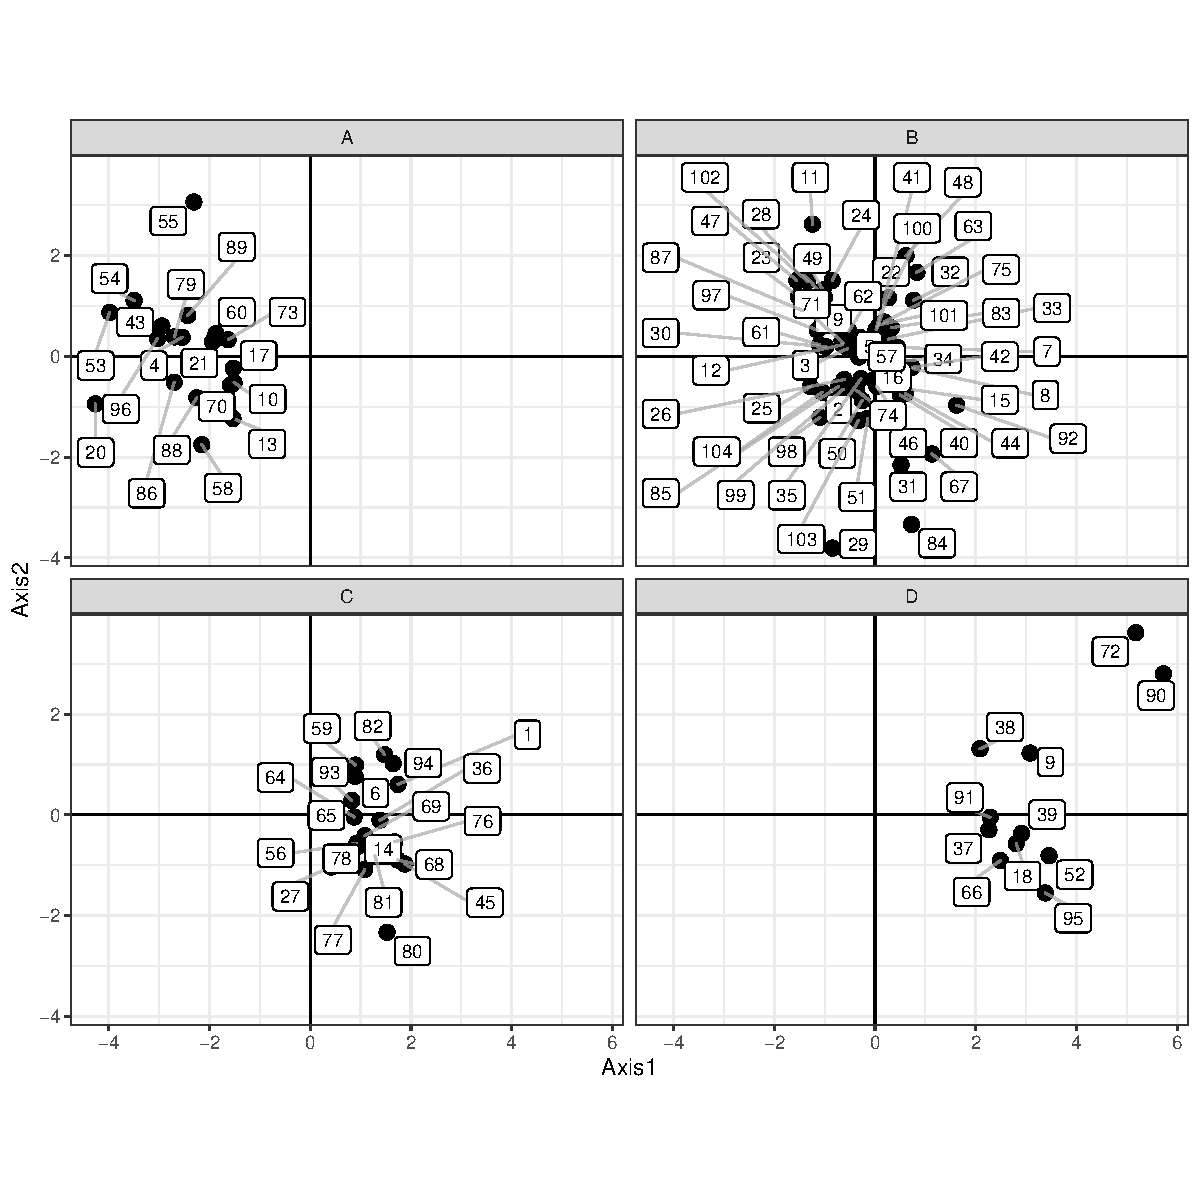
\includegraphics{figs/sweave-liclass1}
\caption{Representation of the observation of the first vectorial plan stratified by group.}
\label{fig:liclass1}
\end{center}
\end{figure}


\begin{figure}[H]
\begin{center}
\begin{Schunk}
\begin{Sinput}
  require(ggplot2)
  require(ggrepel)
  auxi <- deug1$li
  auxi$label <- rownames(auxi)
  auxi$group <- substring(as.character(deug$result),1,1)
  gg <- ggplot(auxi,aes(Axis1,Axis2,label=label,color=group))
  gg <- gg + geom_hline(yintercept = 0) + geom_vline(xintercept = 0)
  gg <- gg + geom_point(shape=19,size=3)
  gg <- gg + geom_label_repel(size = 3,segment.alpha=0.7,segment.color = "darkgrey")
  gg <-  gg + theme_bw() + coord_fixed(ratio=1) + facet_wrap(~ group)
  gg
\end{Sinput}
\end{Schunk}
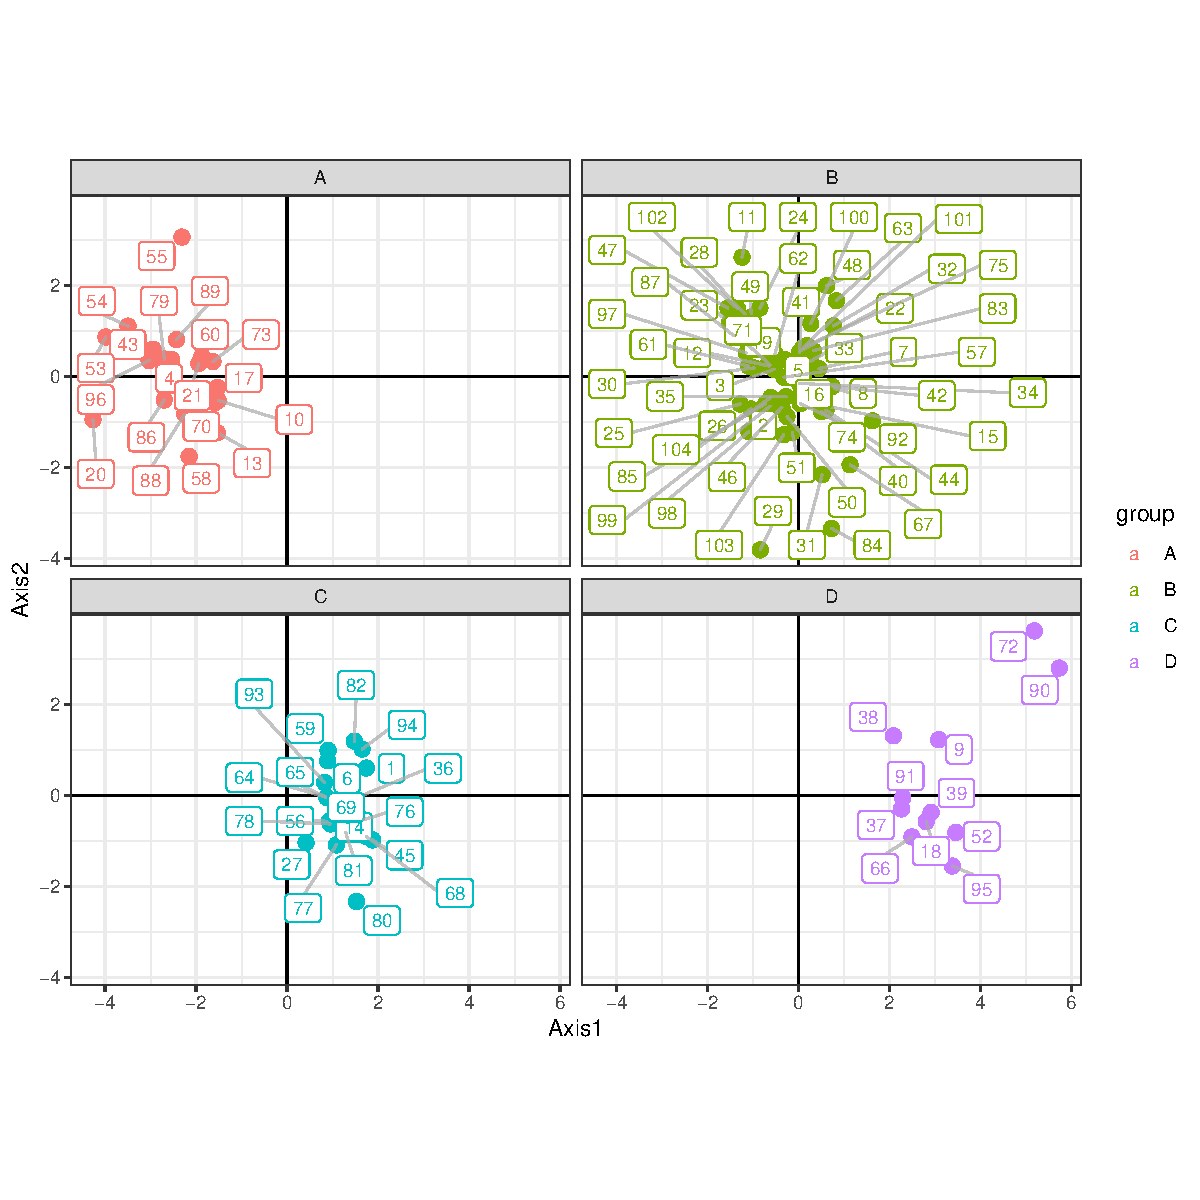
\includegraphics{figs/sweave-liclass2}
\caption{Representation of the observation of the first vectorial plan stratified by group (with color).}
\label{fig:liclass2}
\end{center}
\end{figure}



\subsection{Ellipses}


\begin{figure}[H]
\begin{center}
\begin{Schunk}
\begin{Sinput}
  require(ggplot2)
  require(ggrepel)
  auxi <- deug1$li
  auxi$label <- rownames(auxi)
  auxi$group <- substring(as.character(deug$result),1,1)
  gg <- ggplot(auxi,aes(Axis1,Axis2,label=label,color=group))
  gg <- gg + geom_hline(yintercept = 0) + geom_vline(xintercept = 0)
  gg <- gg + geom_point(shape=19,size=3)
  gg <- gg + stat_ellipse(type = "norm",level=0.66)
  gg <- gg + geom_label_repel(size = 3,segment.alpha=0.7,segment.color = "darkgrey")
  gg <-  gg + theme_bw() + coord_fixed(ratio=1)
  gg
\end{Sinput}
\end{Schunk}
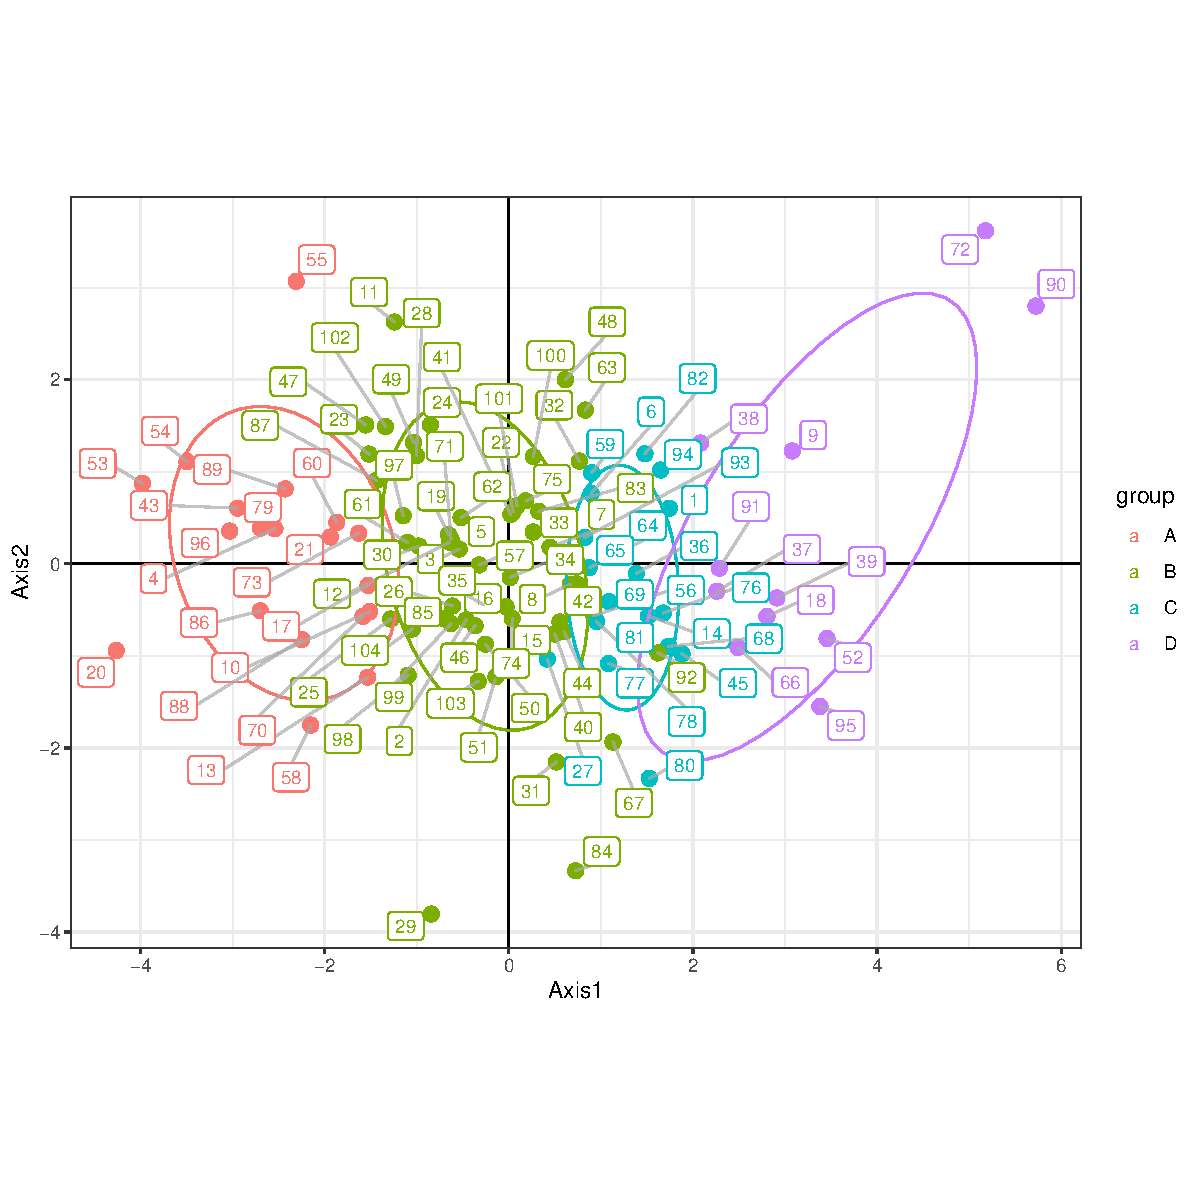
\includegraphics{figs/sweave-liclass3}
\caption{Representation of the observation of the first vectorial plan with ellpise of Inertia for each group}
\label{fig:liclass3}
\end{center}
\end{figure}

\begin{figure}[H]
\begin{center}
\begin{Schunk}
\begin{Sinput}
  require(ggplot2)
  require(ggrepel)
  auxi <- deug1$li
  auxi$label <- rownames(auxi)
  auxi$group <- substring(as.character(deug$result),1,1)
  gg <- ggplot(auxi,aes(Axis1,Axis2,label=label,color=group))
  gg <- gg + geom_hline(yintercept = 0) + geom_vline(xintercept = 0)
  gg <- gg + geom_point(shape=19,size=3)
  gg <- gg + stat_ellipse(type = "norm",level=0.66)
  gg <- gg + geom_label_repel(size = 3,segment.alpha=0.7,segment.color = "darkgrey")
  gg <-  gg + theme_bw() + coord_fixed(ratio=1) + facet_wrap(~group)
  gg
\end{Sinput}
\end{Schunk}
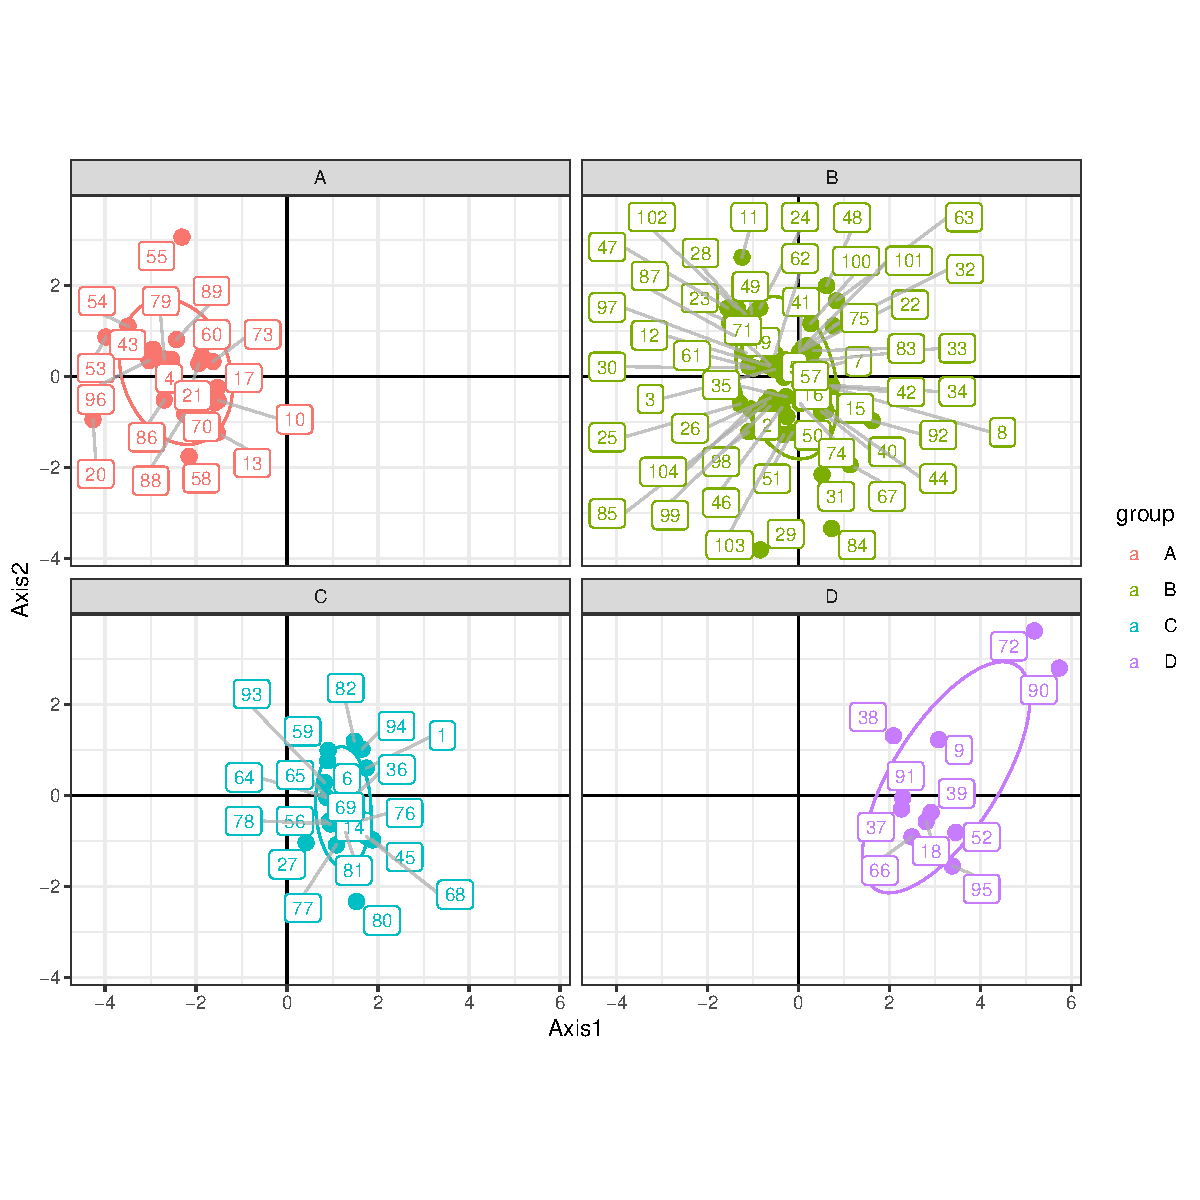
\includegraphics{figs/sweave-liclass4}
\caption{Representation of the observation of the first vectorial plan with ellpise of Inertia for each group}
\label{fig:liclass4}
\end{center}
\end{figure}

\subsection{Ellipses and stars}
For this representation, we need to compute the position of the gravity center of each ellipse. This operation was performed by the R function \texttt{prep.tab.class}. The implementation of this function is given below:

\begin{Schunk}
\begin{Sinput}
  prep.tab.class <- function(x,fac,varnames=c("Axis1","Axis2"),rm.X=TRUE,...){
   x <- as.data.frame(x)
   x$fac <- factor(x[,fac])
   w <- tab.class(x[,varnames],fac=x$fac)
   colnames(w) <- c("Axis1","Axis2")
   if(rm.X){
     w$label <- gsub("X","",rownames(w)) #levels(x$fac)
   }else{
     w$label <- rownames(w)
   }
   rownames(w) <- as.character(w$label)
   x$cAxis1 <- w$Axis1[match(as.character(x$fac),w$label)]
   x$cAxis2 <- w$Axis2[match(as.character(x$fac),w$label)]
   return(list(data=x,center=w))
 }
\end{Sinput}
\end{Schunk}


\begin{figure}[H]
\begin{center}
\begin{Schunk}
\begin{Sinput}
  require(ggplot2)
  require(ggrepel)
  auxi <- deug1$li
  auxi$label <- rownames(auxi)
  auxi$group <- substring(as.character(deug$result),1,1)
  w <- prep.tab.class(auxi,varnames=c("Axis1","Axis2"),fac="group",rm.X=FALSE)
  datax <- w$data
  centerx <- w$center
  gg <- ggplot(datax,aes(x=Axis1,y=Axis2,col=group,group=group)) 
  gg <- gg + geom_hline(yintercept = 0) + geom_vline(xintercept = 0)
  gg <- gg +  stat_ellipse(type = "norm",level=0.66,lwd=1,show.legend = FALSE)
  gg <- gg + geom_segment(data=datax,aes(x=Axis1,y=Axis2, xend = cAxis1, yend = cAxis2))
  gg <- gg + geom_point(data=centerx,aes(x=Axis1,y=Axis2,col=label),inherit.aes = FALSE,size=0)
  gg <- gg + geom_point(shape=19,size=2,show.legend = FALSE)
  # gg <- gg + geom_label_repel(data=centerx,aes(x=Axis1,y=Axis2,col=label,label=label),size = 3,
  #                             segment.alpha=0.7,segment.color = "darkgrey",fontface = 'bold',inherit.aes = FALSE)
  gg <- gg + geom_label(data=centerx,aes(x=Axis1,y=Axis2,col=label,label=label),size = 3,
                             fontface = 'bold',inherit.aes = FALSE)
  gg <- gg + theme_light() +theme(legend.position = "none") + coord_fixed(ratio=1)
  gg
  
\end{Sinput}
\end{Schunk}
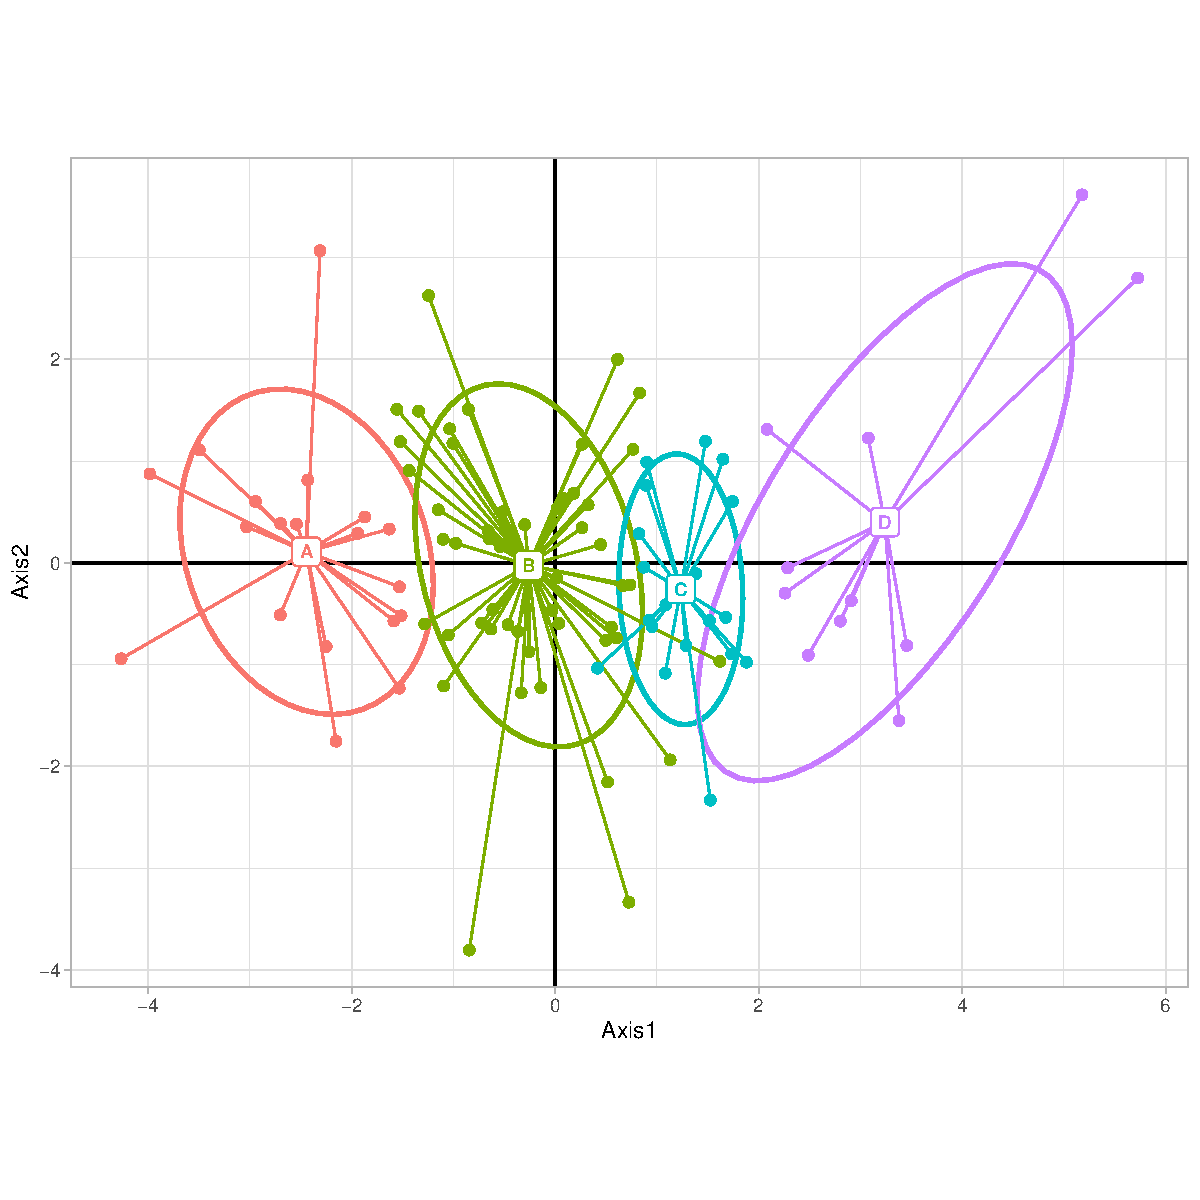
\includegraphics{figs/sweave-liclassSTAR}
\caption{Representation of the observation of the first vectorial plan with ellpise of Inertia for each group}
\label{fig:liclassSTAR}
\end{center}
\end{figure}



\subsection{Chull representation}

The following code is based on the vignette related to the extending ggplot2 functions (https://cran.r-project.org/web/packages/ggplot2/vignettes/extending-ggplot2.htm). The additional functions for the computation necessary to the Convex hull representation are given below:

\begin{Schunk}
\begin{Sinput}
  StatChull <- ggproto("StatChull", Stat,
   compute_group = function(data, scales) {
     data[chull(data$x, data$y), , drop = FALSE]
   },
   
   required_aes = c("x", "y")
 )
  stat_chull <- function(mapping = NULL, data = NULL, geom = "polygon",
                        position = "identity", na.rm = FALSE, show.legend = NA, 
                        inherit.aes = TRUE, ...) {
   layer(
     stat = StatChull, data = data, mapping = mapping, geom = geom, 
     position = position, show.legend = show.legend, inherit.aes = inherit.aes,
     params = list(na.rm = na.rm, ...)
   )
 }
\end{Sinput}
\end{Schunk}

The representation for one group is given below:

\begin{figure}[H]
\begin{center}
\begin{Schunk}
\begin{Sinput}
  require(ggplot2)
  # data 
  auxi <- deug1$li
  auxi$label <- rownames(auxi)
  auxi$group <- substring(as.character(deug$result),1,1)
  # Find the convex hull of the points being plotted
  # Define the scatterplot
  gg <- ggplot(auxi,aes(Axis1,Axis2,col=group))
  gg <- gg + geom_hline(yintercept = 0) + geom_vline(xintercept = 0)
  gg <- gg + geom_point(shape=19,size=3)
  gg <- gg + stat_chull(fill=NA)
  gg <-  gg + theme_bw() + coord_fixed(ratio=1)
  gg
\end{Sinput}
\end{Schunk}
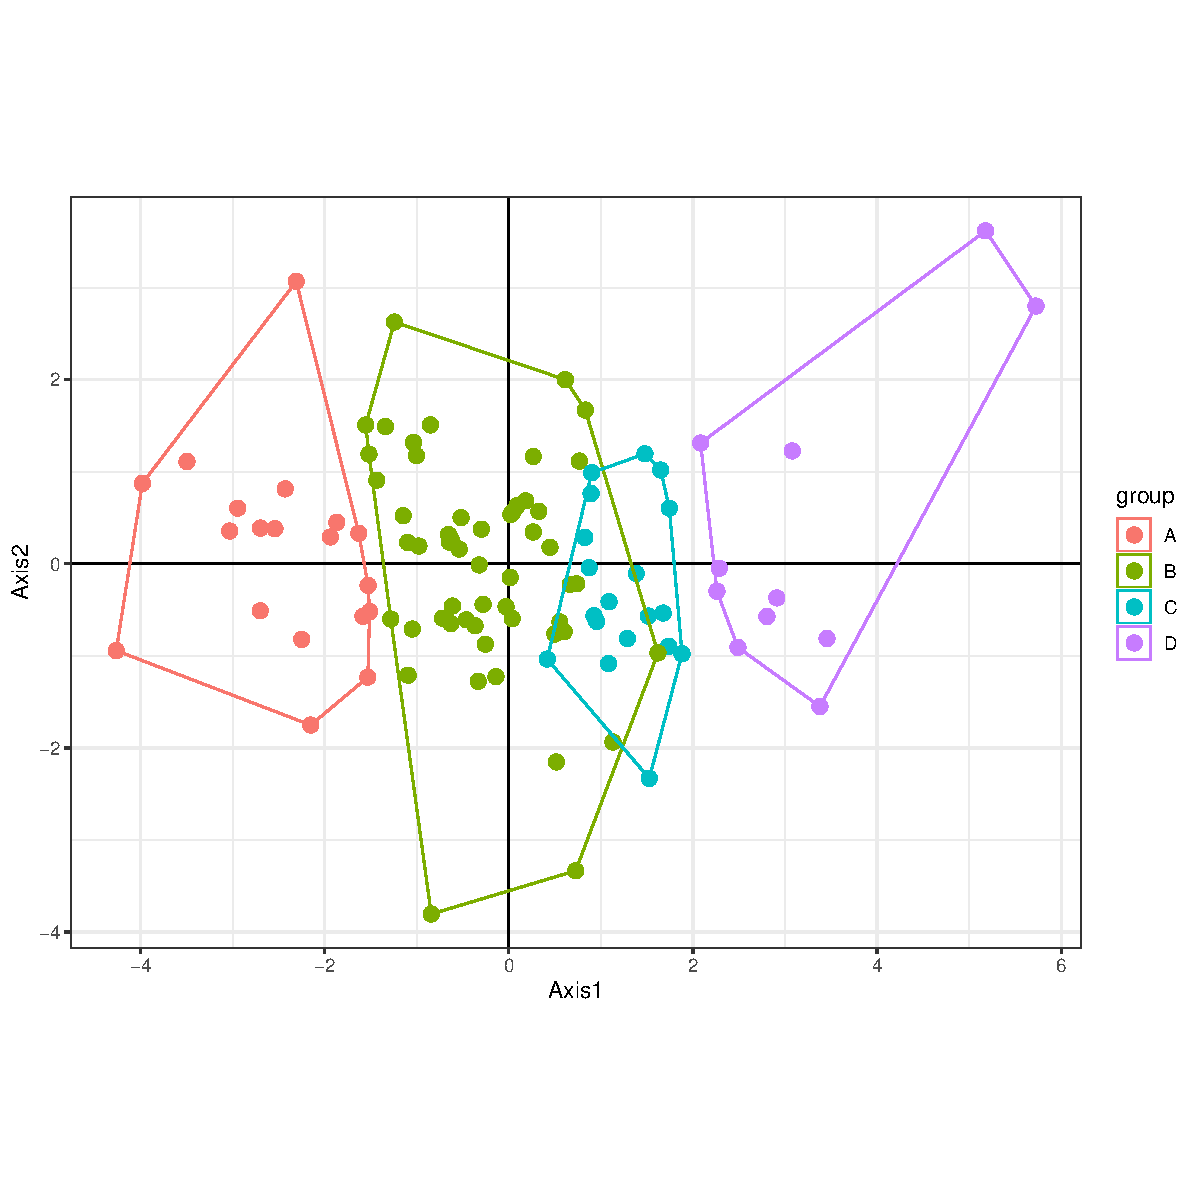
\includegraphics{figs/sweave-lichull1}
\caption{Chull representation of the observation of the first vectorial plan.}
\label{fig:lichull1}
\end{center}
\end{figure}


\begin{figure}[H]
\begin{center}
\begin{Schunk}
\begin{Sinput}
  require(ggplot2)
  # data 
  auxi <- deug1$li
  auxi$label <- rownames(auxi)
  auxi$group <- substring(as.character(deug$result),1,1)
  # Find the convex hull of the points being plotted
  # Define the scatterplot
  gg <- ggplot(auxi,aes(Axis1,Axis2,col=group,fill=group))
  gg <- gg + geom_hline(yintercept = 0) + geom_vline(xintercept = 0)
  gg <- gg + geom_point(shape=19,size=3)
  gg <- gg + stat_chull(alpha=0.5)
  gg <-  gg + theme_bw() + coord_fixed(ratio=1)
  gg
\end{Sinput}
\end{Schunk}
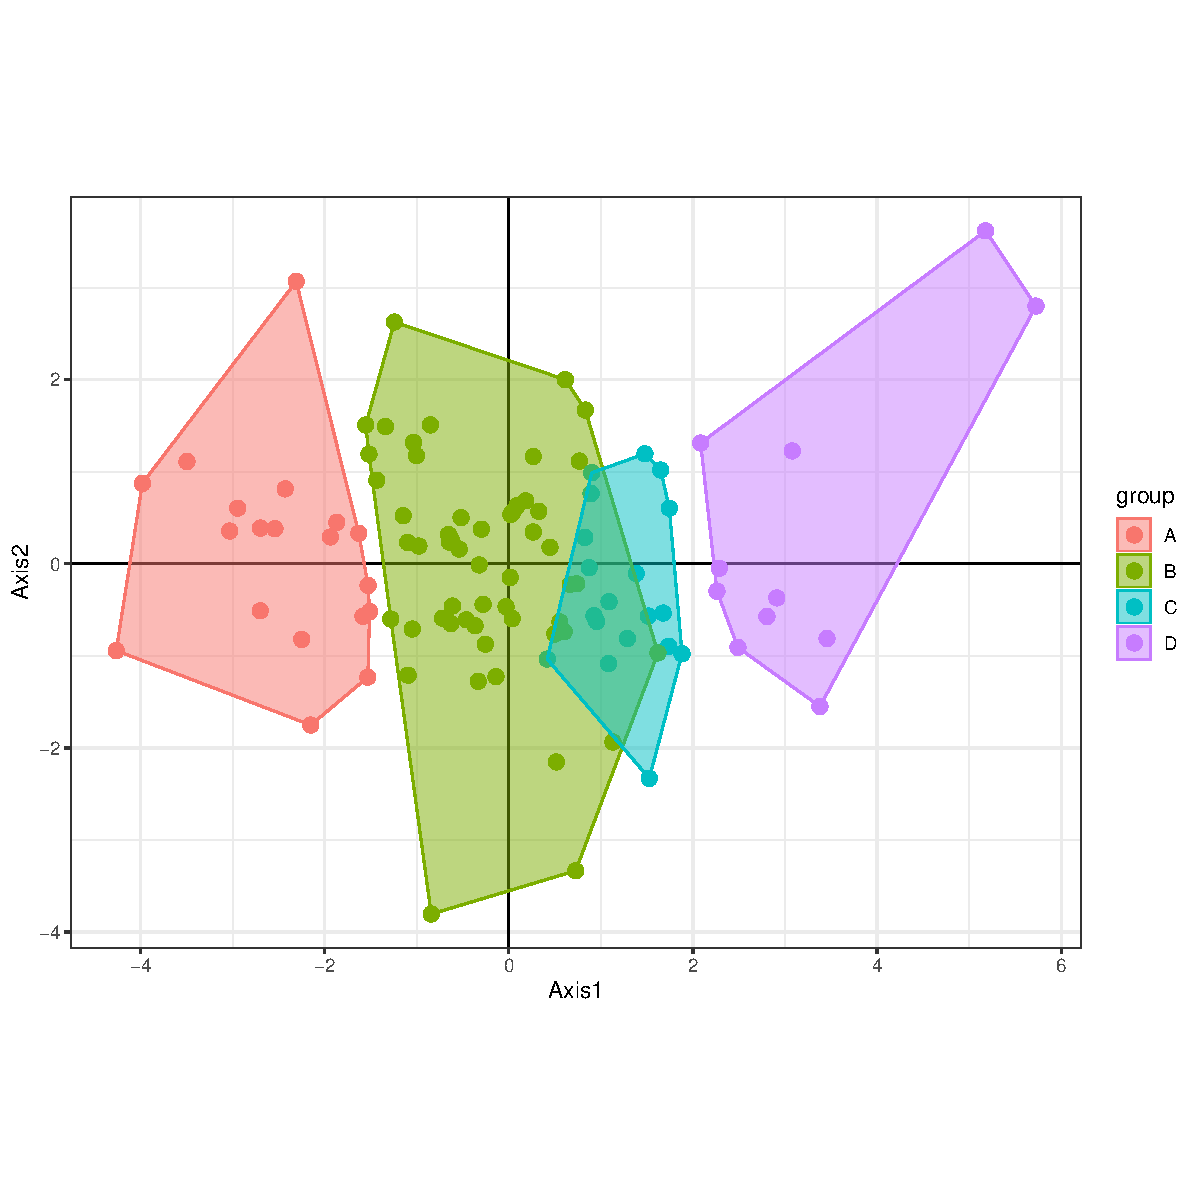
\includegraphics{figs/sweave-lichull2}
\caption{Chull representation of the observation of the first vectorial plan.}
\label{fig:lichull2}
\end{center}
\end{figure}



\section{2D density}

\begin{figure}[H]
\begin{center}
\begin{Schunk}
\begin{Sinput}
  require(ggplot2)
  require(ggrepel)
  auxi <- deug1$li
  auxi$label <- rownames(auxi)
  auxi$group <- deug$result
  gg <- ggplot(auxi,aes(Axis1,Axis2,label=label))
  gg <- gg + geom_hline(yintercept = 0) + geom_vline(xintercept = 0)
  gg <- gg + geom_point(shape=19,size=3)
  gg <- gg + stat_density2d(col="blue")
  gg <-  gg + theme_bw() + coord_fixed(ratio=1)
  gg
\end{Sinput}
\end{Schunk}
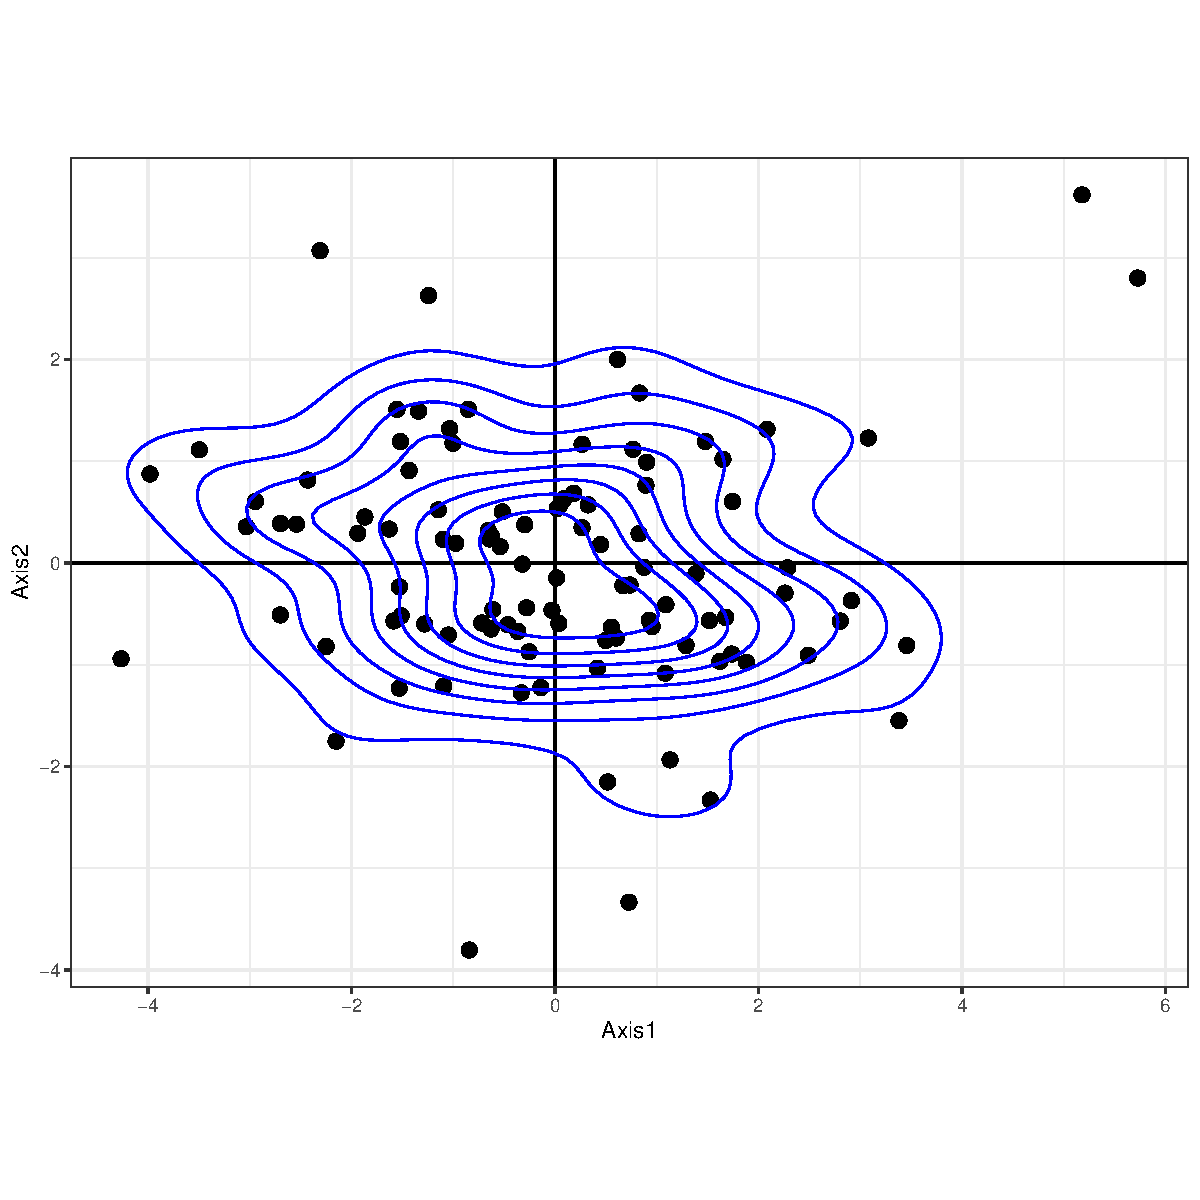
\includegraphics{figs/sweave-lidensity1}
\caption{Representation of the observation with 2-D kernel density}
\label{fig:lidensity1}
\end{center}
\end{figure}



\begin{figure}[H]
\begin{center}
\begin{Schunk}
\begin{Sinput}
  require(ggplot2)
  require(ggrepel)
  auxi <- deug1$li
  auxi$label <- rownames(auxi)
  auxi$group <- substring(as.character(deug$result),1,1)
  gg <- ggplot(auxi,aes(Axis1,Axis2,label=label,col=group))
  gg <- gg + geom_hline(yintercept = 0) + geom_vline(xintercept = 0)
  gg <- gg + geom_point(shape=19,size=3)
  gg <- gg + stat_density2d(col="blue")
  gg <-  gg + theme_bw() + coord_fixed(ratio=1)
  gg
\end{Sinput}
\end{Schunk}
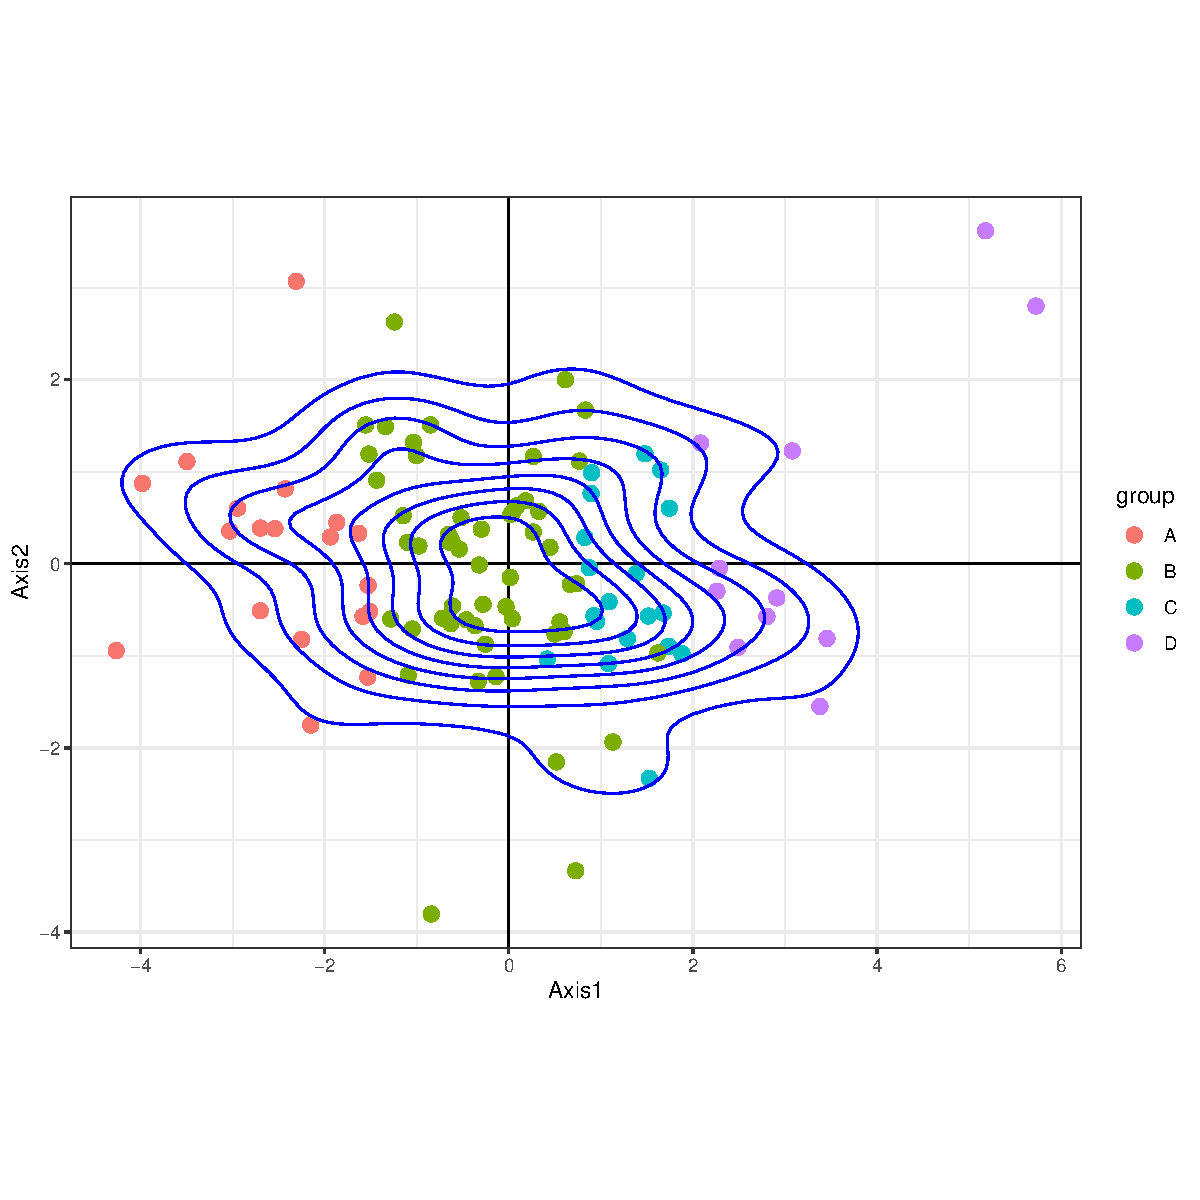
\includegraphics{figs/sweave-lidensity2}
\caption{Representation of the observation with 2-D kernel density}
\label{fig:lidensity2}
\end{center}
\end{figure}



\begin{figure}[H]
\begin{center}
\begin{Schunk}
\begin{Sinput}
  require(ggplot2)
  require(ggrepel)
  auxi <- deug1$li
  auxi$label <- rownames(auxi)
  auxi$group <- substring(as.character(deug$result),1,1)
  gg <- ggplot(auxi,aes(Axis1,Axis2,label=label,col=group))
  gg <- gg + geom_hline(yintercept = 0) + geom_vline(xintercept = 0)
  gg <- gg + geom_point(shape=19,size=3)
  gg <- gg + stat_density2d(col="blue")
  gg <-  gg + theme_bw() + coord_fixed(ratio=1) + facet_wrap(~group)
  gg
\end{Sinput}
\end{Schunk}
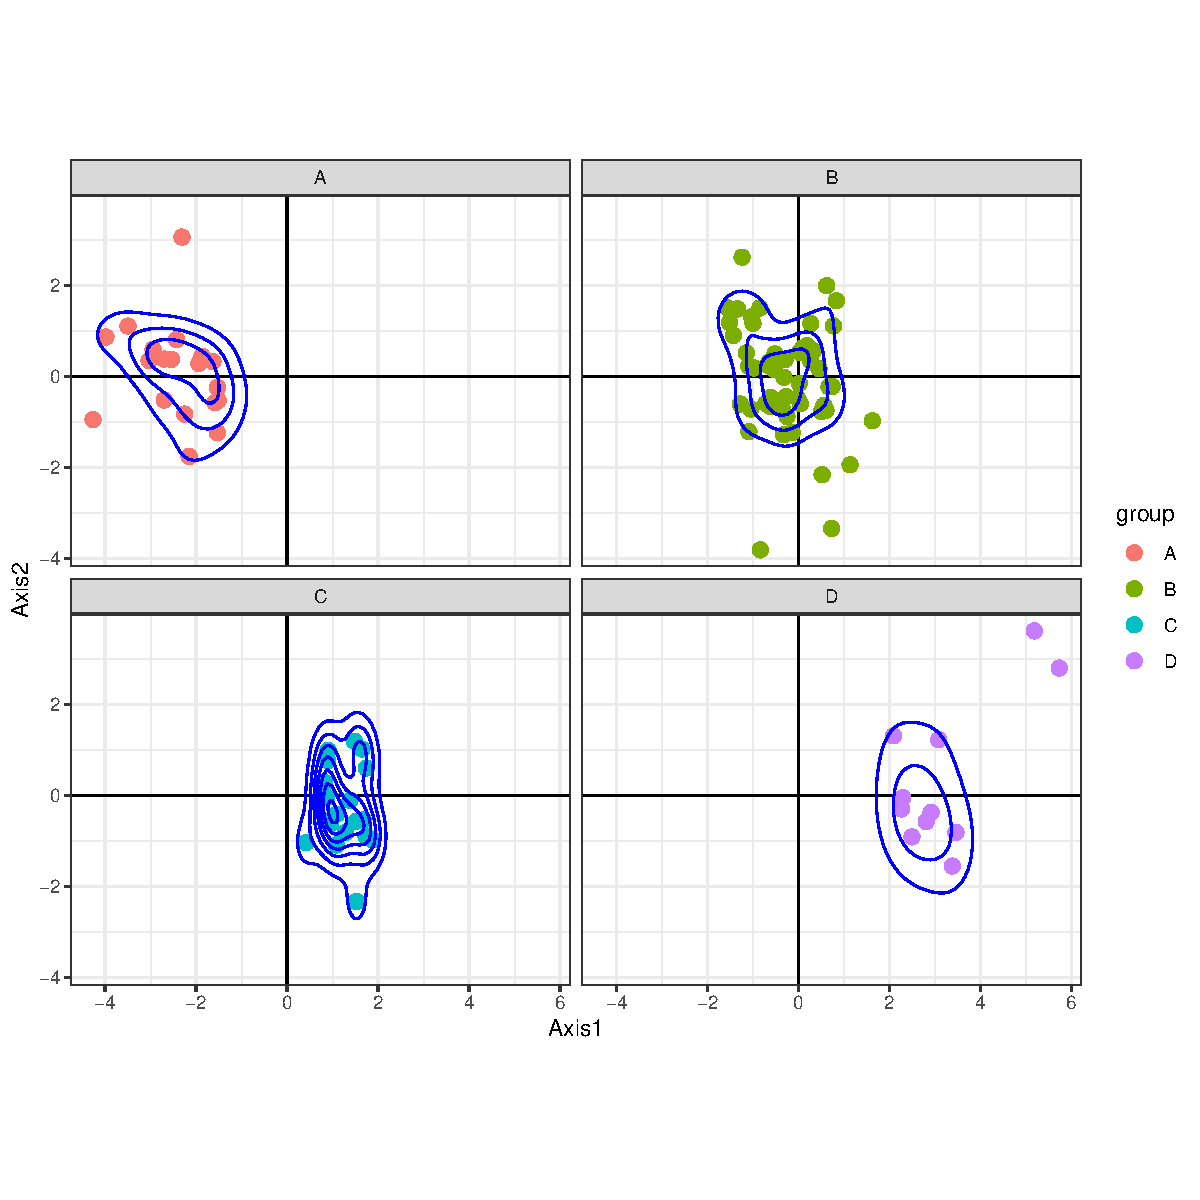
\includegraphics{figs/sweave-lidensity3}
\caption{Representation of the observation with 2-D kernel density}
\label{fig:lidensity3}
\end{center}
\end{figure}



\section{Adding a picture}

The functions from the R package imager (\cite{imager}) can be used To add picture on ggplot graphics (\url{https://cran.r-project.org/web/packages/imager/vignettes/gettingstarted.html}).
\begin{figure}[H]
\begin{center}
\begin{Schunk}
\begin{Sinput}
  library(ggplot2)
  library(dplyr)
  library(imager)
  parrots <- load.image("/export/scratch/R/library/imager/extdata/parrots.png")
  df <- as.data.frame(parrots,wide="c") %>% mutate(rgb.val=rgb(c.1,c.2,c.3))
  df$y <- rev(df$y)
  gg <- ggplot(df,aes(x,y)) + geom_raster(aes(fill=rgb.val)) + scale_fill_identity()
  gg <- gg + xlab("x") + ylab("y")
  gg <- gg + theme_bw()  + coord_fixed(ratio=1)
  gg
\end{Sinput}
\end{Schunk}
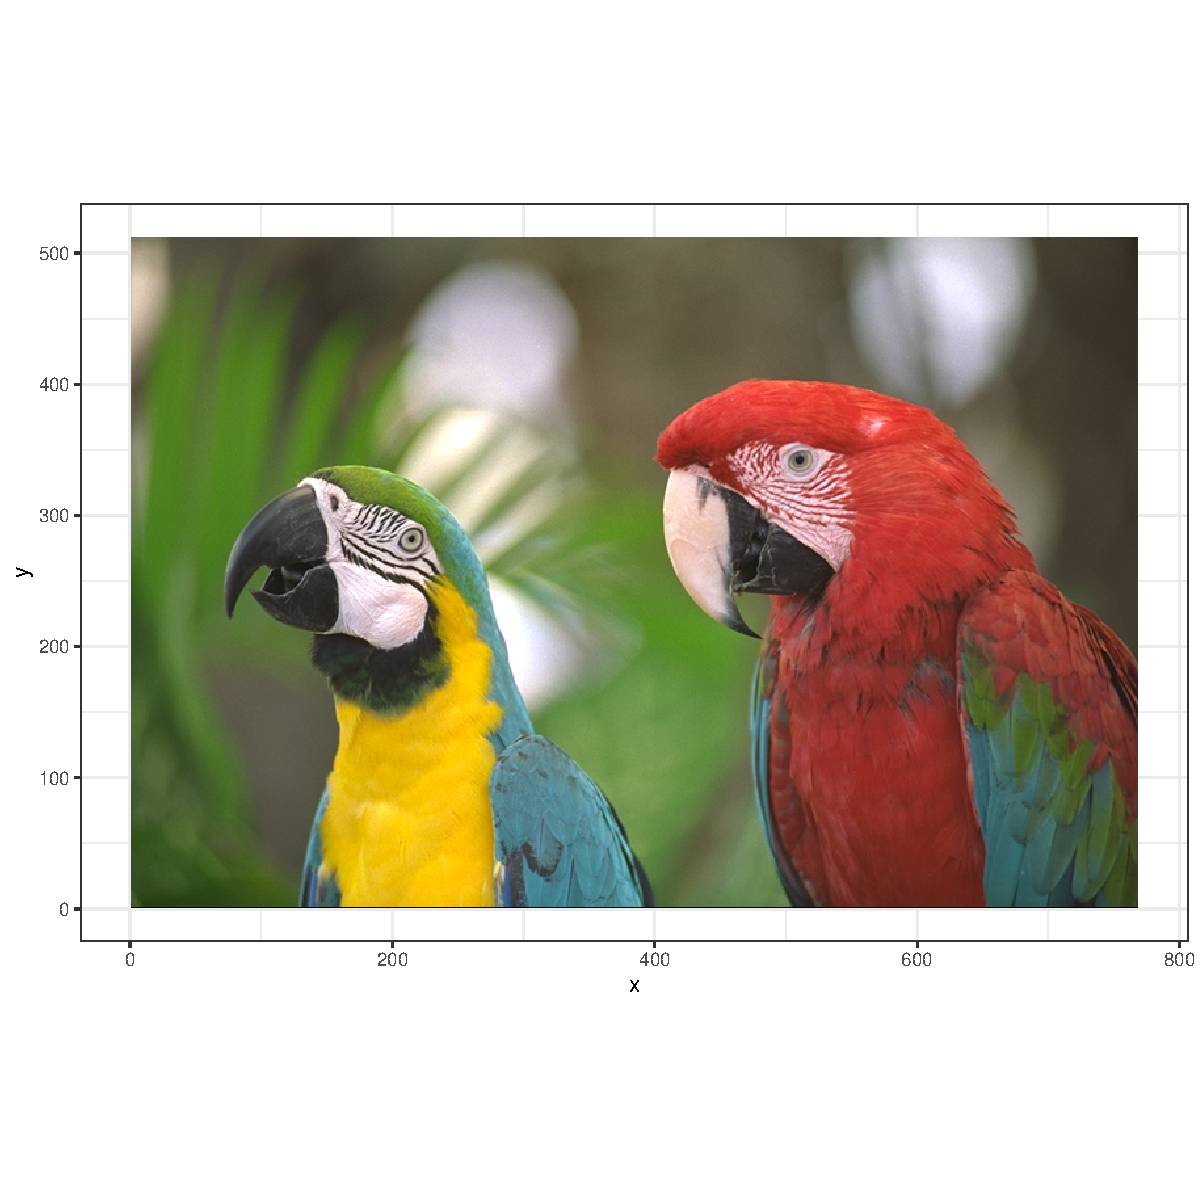
\includegraphics{figs/sweave-image1}
\caption{Representation of "parrots" picture from R package \texttt{imager}.}
\label{fig:image1}
\end{center}
\end{figure}



Test for PNM format with imager ... resultats boff (?!)
\begin{figure}[H]
\begin{center}
\begin{Schunk}
\begin{Sinput}
  library(ggplot2)
  library(dplyr)
  library(imager)
  #photo1 <- load.image("/export/scratch/R/library/ade4/inst/pictures/buterfly.pnm")
  maps1 <- load.image("/export/scratch/R/library/ade4/pictures/butterfly.pnm")
  df <- as.data.frame(maps1)
  # black=#000000 and white = #FFFFFF
  df$rgb.val <- ifelse(df$value==0,'#000000','#FFFFFF')
  df$y <- rev(df$y)
  gg <- ggplot(df,aes(x,y)) + geom_raster(aes(fill=rgb.val)) + scale_fill_identity()
  gg <- gg + xlab("x") + ylab("y")
  gg <- gg + theme_bw()  + coord_fixed(ratio=1)
  gg
\end{Sinput}
\end{Schunk}
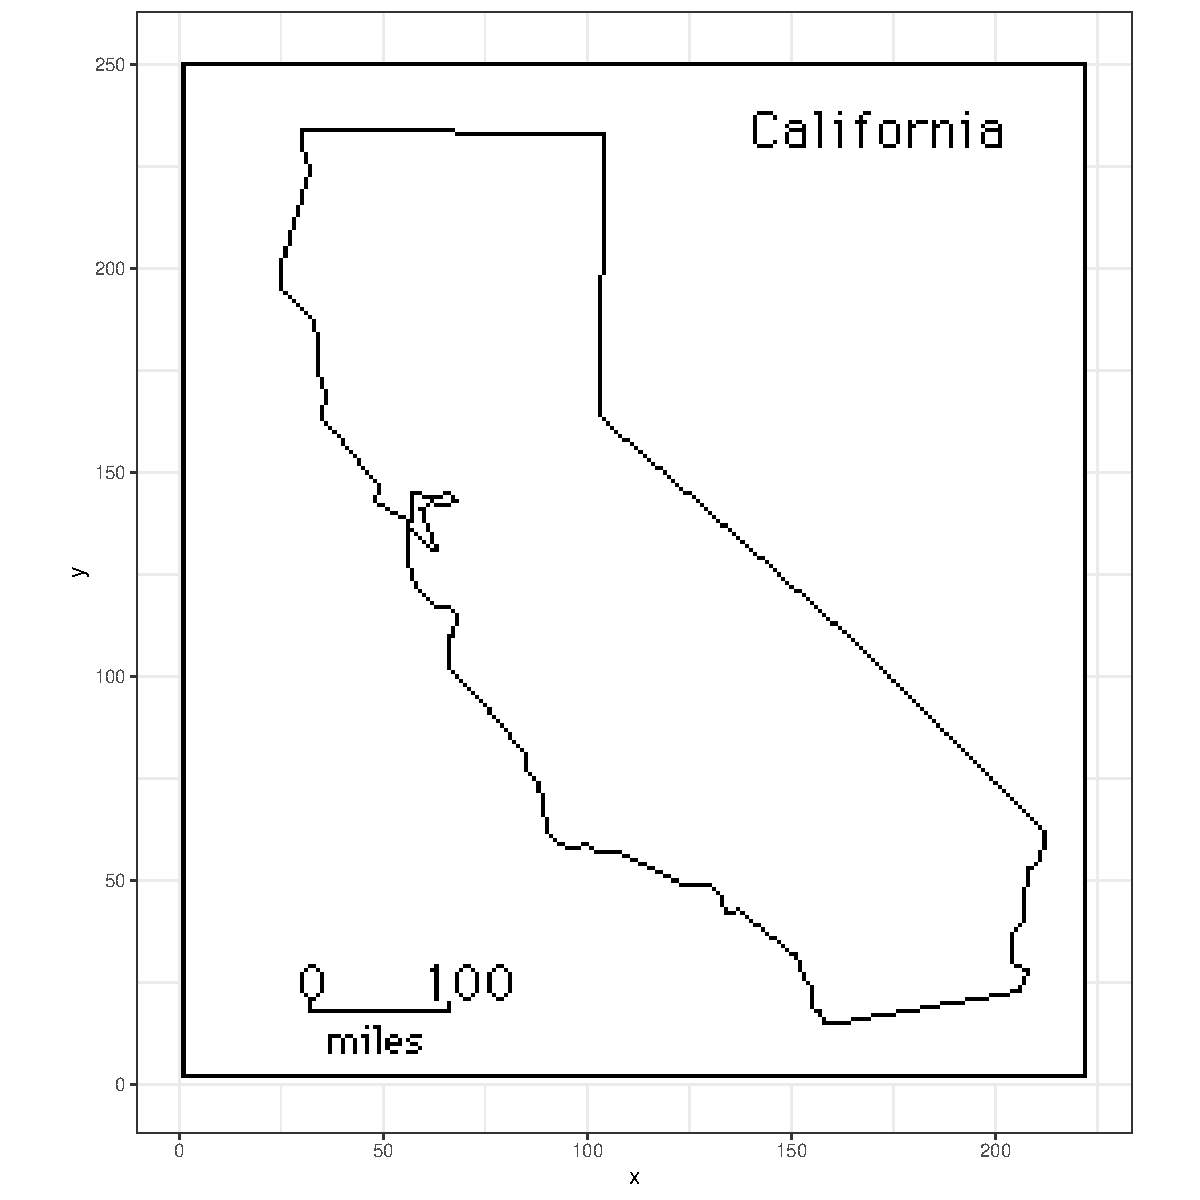
\includegraphics{figs/sweave-image2}
\caption{Representation of the map associated with butterfly data from R package \texttt{ade4}.}
\label{fig:image2}
\end{center}
\end{figure}

For the color code see https://www.nceas.ucsb.edu/sites/default/files/2020-04/colorPaletteCheatsheet.pdf. The previous results is not very good. we try to used the R package \texttt{magick} https://docs.ropensci.org/magick/articles/intro.html). The code is given below:

\begin{Schunk}
\begin{Sinput}
  require(magick)
  maps2 <-  image_read("/export/scratch/R/library/ade4/pictures/butterfly.pnm") 
\end{Sinput}
\end{Schunk}

add points and information
\begin{figure}[H]
\begin{center}
\begin{Schunk}
\begin{Sinput}
  data(butterfly)
  gg <- ggplot(butterfly$xy,aes(x,y)) 
  gg <- gg + annotation_raster(as.raster(maps2),xmin=0,xmax=222,
                          ymin=0,ymax=250,interpolate = TRUE)
  gg <- gg + geom_point()
  gg <- gg + xlab("x") + ylab("y")
  gg <- gg + theme_bw()  + coord_fixed(ratio=1) 
  gg <- gg + scale_y_continuous(limits=c(0,250)) 
  gg <- gg + scale_x_continuous(limits=c(0,222))
  gg
\end{Sinput}
\end{Schunk}
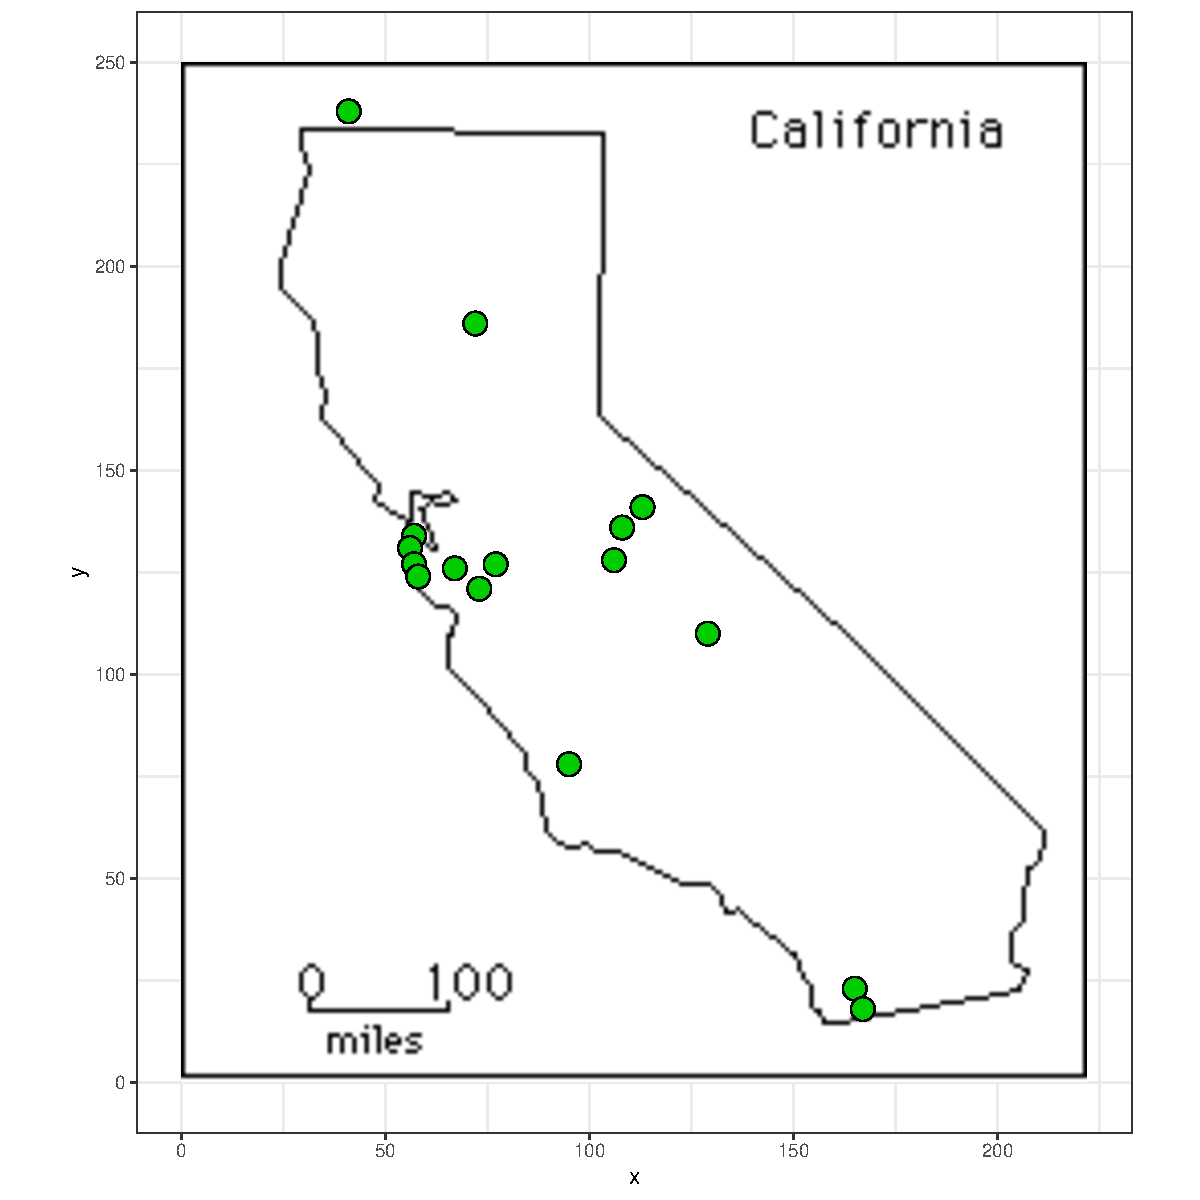
\includegraphics{figs/sweave-image4}
\caption{Representation of the map associated with butterfly data from R package \texttt{ade4}.}
\label{fig:image4}
\end{center}
\end{figure}


\section{Complex figures and Examples}

The complex figures are aggregated with the package \texttt{cowplot} (\cite{cowplot}).

\subsection{Heatmap and PCA}




\subsection{Coinertia analysis}




\subsection{K-table representations}






\section{Conclusion}


\bibliographystyle{plain}
\bibliography{ggade4bib}

\section{Appendix}

\begin{Schunk}
\begin{Sinput}
  print(sessionInfo(),locale=FALSE)
\end{Sinput}
\begin{Soutput}
R version 3.6.3 (2020-02-29)
Platform: x86_64-pc-linux-gnu (64-bit)
Running under: Linux Mint 18.3

Matrix products: default
BLAS:   /usr/lib/openblas-base/libblas.so.3
LAPACK: /usr/lib/libopenblasp-r0.2.18.so

Random number generation:
 RNG:     Mersenne-Twister 
 Normal:  Inversion 
 Sample:  Rounding 
 
attached base packages:
 [1] datasets  parallel  stats     graphics  utils     stats4    tools     grDevices
 [9] methods   base     

other attached packages:
 [1] magick_2.0           imager_0.41.2        magrittr_1.5        
 [4] dplyr_1.0.2          ggforce_0.2.2        ggrepel_0.8.1       
 [7] cowplot_0.9.4        ggplot2_3.3.2        knitr_1.23          
[10] pixmap_0.4-11        ade4_1.7-15          RColorBrewer_1.1-2  
[13] rtracklayer_1.44.0   GenomicRanges_1.36.0 GenomeInfoDb_1.20.0 
[16] IRanges_2.18.0       S4Vectors_0.22.1     BiocGenerics_0.30.0 

loaded via a namespace (and not attached):
 [1] Rcpp_1.0.5                  lattice_0.20-38            
 [3] png_0.1-7                   Rsamtools_2.0.0            
 [5] Biostrings_2.52.0           digest_0.6.22              
 [7] R6_2.4.0                    tiff_0.1-5                 
 [9] plyr_1.8.4                  pillar_1.4.7               
[11] zlibbioc_1.30.0             rlang_0.4.9                
[13] rstudioapi_0.10             Matrix_1.2-17              
[15] bmp_0.3                     labeling_0.3               
[17] BiocParallel_1.18.1         stringr_1.4.0              
[19] igraph_1.2.4.1              RCurl_1.95-4.12            
[21] polyclip_1.10-0             munsell_0.5.0              
[23] DelayedArray_0.10.0         compiler_3.6.3             
[25] xfun_0.10                   pkgconfig_2.0.3            
[27] readbitmap_0.1.5            tidyselect_1.1.0           
[29] SummarizedExperiment_1.14.0 tibble_3.0.4               
[31] GenomeInfoDbData_1.2.1      matrixStats_0.55.0         
[33] XML_3.98-1.20               crayon_1.3.4               
[35] withr_2.1.2                 GenomicAlignments_1.20.0   
[37] MASS_7.3-51.4               bitops_1.0-6               
[39] grid_3.6.3                  gtable_0.3.0               
[41] lifecycle_0.2.0             scales_1.0.0               
[43] stringi_1.4.3               farver_1.1.0               
[45] XVector_0.24.0              ellipsis_0.3.0             
[47] generics_0.0.2              vctrs_0.3.5                
[49] Biobase_2.44.0              glue_1.4.2                 
[51] tweenr_1.0.1                purrr_0.3.4                
[53] jpeg_0.1-8.1                colorspace_1.4-1           
[55] isoband_0.2.3              
\end{Soutput}
\begin{Sinput}
  options(encoding="latin1",prompt=">  ", continue=" ", width = 85)
>  #save.image()
\end{Sinput}
\end{Schunk}

\end{document}
